\documentclass[12pt]{article}
\usepackage{sbc-template}
\usepackage{graphicx,url}
\usepackage[utf8]{inputenc}
\usepackage[brazil]{babel}
\usepackage{color}
\usepackage{listings}

%%%%%%%%%%%%%%%%%%%%%%%%%%%%%%%%%%%%%%%%%%%%%%%%%%%%
% C O N F I G U R A Ç Õ E S  D O S   C Ó D I G O S %
%%%%%%%%%%%%%%%%%%%%%%%%%%%%%%%%%%%%%%%%%%%%%%%%%%%%

\lstset{
	numbers=left,
	stepnumber=1,
	firstnumber=1,
	numberstyle=\scriptsize,
	extendedchars=true,
	breaklines=true,
	frame=single,
	showstringspaces=false,
  aboveskip=1.5em,
	xleftmargin=2.5em,
	framexleftmargin=2em,
	basicstyle=\scriptsize,
}

\renewcommand{\lstlistingname}{Código}
\renewcommand{\lstlistlistingname}{Lista de Códigos}

\sloppy

\title{Aprendizagem de Máquina (2020/Período Especial) - Redes Neurais}

\author{Diogo C. T. Batista\inst{1}}

\address{Universidade Federal do Paraná (UFPR)\\
	Curitiba -- Paraná -- Brasil
	\email{diogo@diogocezar.com}
	}

\begin{document}

\maketitle

\section{Introdução}

Neste laboratório, foi considerada uma base de dados com os meses do ano. As imagens são representações manuscritas das palavras que compreendem os meses: Janeiro, Fevereiro, Março, Abril, Maio, Junho, Julho, Agosto, Setembro, Outubro, Novembro e Dezembro. Portanto, são 12 classes. A Figura \ref{fig:image_months} demostra alguns exemplos dessas imagens.

\begin{figure}[!htb]
  \centering
  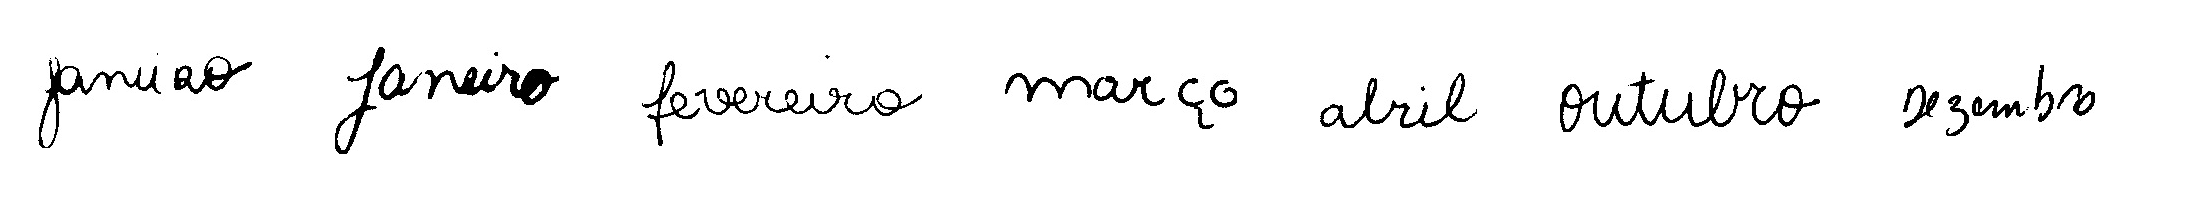
\includegraphics[width=35em]{images/image_months.png}
  \caption{Exemplos dos meses manuscritos}
  \label{fig:image_months}
\end{figure}

As implementações para este laboratório foram relaizadas na plataforma \textit{Google Colab}. Para a obtenção dos resultados explorados neste trabalho, foram realizadas as seguintes etapas: \textit{Preparações}, \textit{Definição dos Modelos}, \textit{Execução do Modelo LeNet5 sem Data Augmentation}, \textit{Execução de um Modelo Personalizado sem Data Augmentation}, \textit{Implementação de Data Augmentation}, \textit{Execução do Modelo LeNet5 com Data Augmentation}, \textit{Execução de um Modelo Personalizado com Data Augmentation}, \textit{Extração de Características} e \textit{Implementação do SVM com as Características Extraídas}.

Cada uma das etapas será detalhada na sequência. Para cada uma das etapas, apresenta-se os resultados obtidos. Ao final do trabalho discute-se os resultados encontrados.

Para a execução dos experimentos, utilizou-se os \textit{frameworks} \textbf{Keras} e \textbf{Sklearn}.

\section{Preparações}

Na estapa de preparação, foram realizadas as implementações que possibilitaram:

\begin{enumerate}
  \item habilitação da GPU;
  \item importação dos dados hospedados no GitHub;
  \item definição dos arquivos de entrada;
  \item definição das funções auxiliares;
\end{enumerate}

Ao executar os experimentos na plataforma Colab do Google, foi possível trabalhar com o processamento via GPU;

Na definição das funções auxiliares, o objetivo foi definir os possíveis componentes reutilizáveis nos experimentos, encapsulando implementações em funções reutilizáveis, além de reduzir a complexidade das implementações, deixando os códigos mais legíveis.

\section{Definição dos Modelos}

Na etapa de definição dos modelos, criou-se a partir do \textit{frameworks} Keras funções que retornam os modelos. Foram definidos dois modelos. O primeiro modelo definido foi o \textit{LeNet5}. Suas camadas estão representadas na Figura \ref{fig:image_lenet5}.

\begin{figure}[!htb]
  \centering
  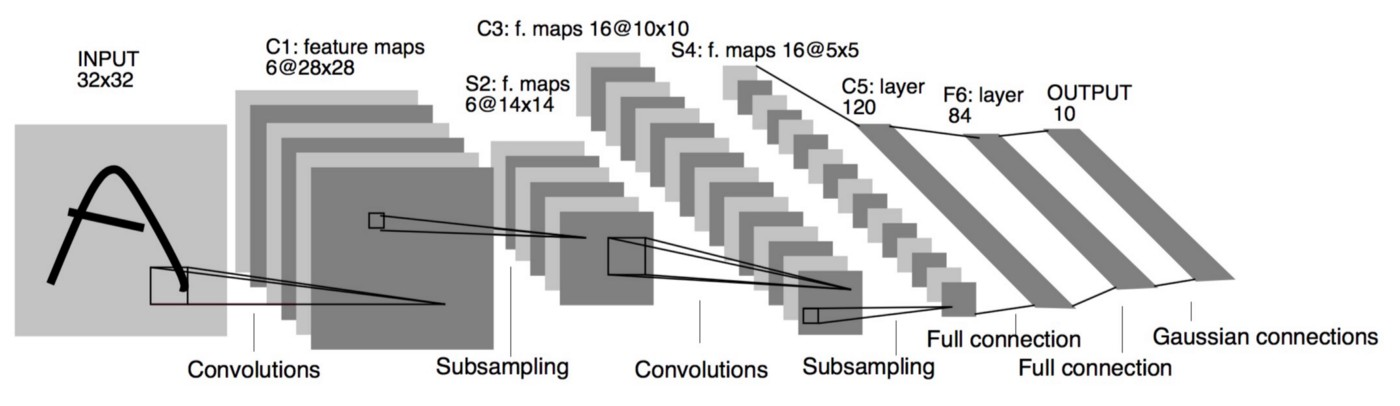
\includegraphics[width=35em]{images/image_lenet.jpeg}
  \caption{Camadas utilizadas pelo modelo LeNet5}
  \label{fig:image_lenet5}
\end{figure}

Este modelo foi usado em grande escala para classificar automaticamente dígitos escritos à mão em cheques bancários nos Estados Unidos. Possui apenas 7 camadas, entre as quais existem 3 camadas convolucionais (C1, C3 e C5), 2 camadas de subamostragem (agrupamento) (S2 e S4) e 1 camada totalmente conectada (F6), que são seguidas pela saída camada. Camadas convolucionais usam 5 por 5 convoluções com passo 1. As camadas de subamostragem são 2 por 2 camadas de pooling médias. As ativações sigmóides de Tanh são usadas em toda a rede. Existem várias opções arquitetônicas interessantes feitas no LeNet-5 que não são muito comuns na era moderna de aprendizado profundo.

O segundo modelo, é o mesmo utilizado nas demonstrações em aula e implementa as seguintes as camadas detalhadas no Código \ref{code:modelo_personalizado}.

\begin{lstlisting}[caption={Modelo Personalizado},captionpos=b,frame=single,label={code:modelo_personalizado}]
model = Sequential()
model.add(Conv2D(32, kernel_size=(3, 3), activation='relu', input_shape=(img_rows,img_cols,3)))
model.add(Conv2D(64, (3, 3), activation='relu'))
model.add(MaxPooling2D(pool_size=(2, 2)))
model.add(Dropout(0.25))
model.add(Flatten())
model.add(Dense(128, activation='relu'))
model.add(Dropout(0.5))
model.add(Dense(num_classes, activation='softmax'))
\end{lstlisting}

Neste modelo, também simplificado, temos 2 convoluções iniciais do tipo \textit{Relu}.
Seguida das operações de \textit{MaxPooling2D}, \textit{Dropout}, \textit{Flatten}, \textit{Dense}, \textit{Dropout} e \textit{Dense}.

\section{Definindo as Execuções}

Quanto ao tamanho da imagem de entrada, para o modelo \textit{LeNet5} utilizou-se o tamanho de 32 por 32 \textit{pixels}, assim como o modelo prevê. Para o modelo \textit{Personalizado} utilizou-se imagens do tamanho 64 por 64 \textit{pixels}.

Com relação ao número de épocas, realizou-se os experimentos com as variações: 32, 64 e 128.

Para todos os experimentos, o tempo de execução em segundos foi registrado.

Para ambos os modelos, realizou-se os seguintes passos:

\begin{enumerate}
  \item carregamento inicial dos dados (x\_train, y\_train, x\_test, y\_test); neste ponto, uma função genérica faz os ajustes necessários nas imagens e retorna os vetores;
  \item normalização das imagens;
  \item geração dos labels para a matriz de confusão;
  \item conversão dos vetores para matrizes binárias;
  \item definição e sumarização do modelo;
  \item compilação do modelo;
  \item treinamento da Rede;
  \item obtenção dos resultados.
\end{enumerate}

Os experimentos foram definidos como:

\begin{itemize}
  \item lenet5\_noaug\_32
  \item lenet5\_noaug\_64
  \item lenet5\_noaug\_128
  \item default\_noaug\_32
  \item default\_noaug\_64
  \item default\_noaug\_128
  \item lenet5\_aug\_32
  \item lenet5\_aug\_64
  \item lenet5\_aug\_128
  \item default\_aug\_32
  \item default\_aug\_64
  \item default\_aug\_128
\end{itemize}

Nos nomes dos experimentos, lenet5 ou default indicam o modelo executado. aug ou noaug indicam no experimento foi utilizada a técnica de data augmentation, ou não. Por fim, os números no final do experimento, indicam a quantidade de épocas testada.

\newpage

\subsection{lenet5\_noaug\_32}

Após a execução deste experimento, obteve-se o gráfico de evolução da acurácia (Figura \ref{fig:experiment_lenet5_noaug_32_accuracy}), o gráfico de perda durante o treinamento (Figura \ref{fig:experiment_lenet5_noaug_32_loss}) e a representação da matriz de confusão (Figura \ref{fig:experiment_lenet5_noaug_32_confusion_matrix}). A Tabela \ref{tab:experiment_lenet5_noaug_32_reults} sumariza os resultados obtidos.

\begin{figure}[!htb]
  \begin{minipage}{.47\textwidth}
    \centering
    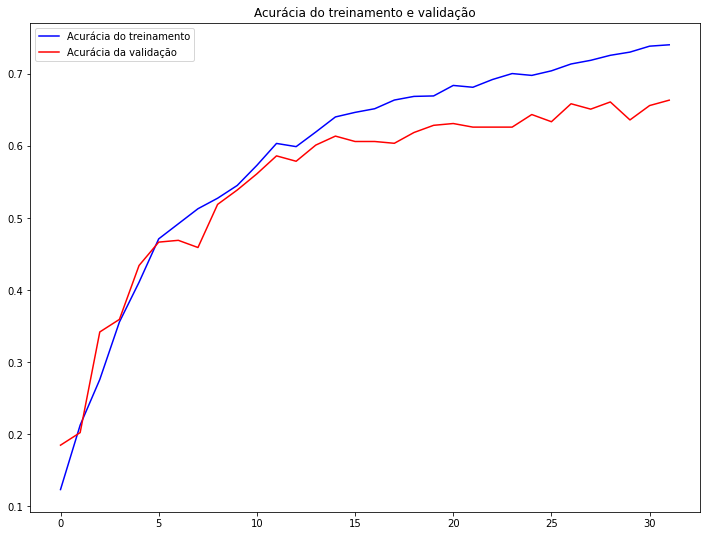
\includegraphics[width=1.1\linewidth]{experiments/lenet5_noaug_32/accuracy.png}
    \caption{Acurácia}\label{fig:experiment_lenet5_noaug_32_accuracy}
  \end{minipage}\hfill
  \begin{minipage}{.47\textwidth}
    \centering
    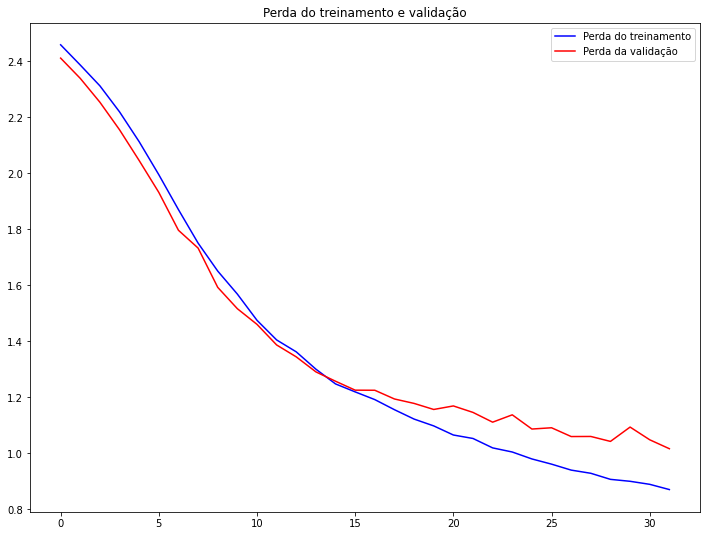
\includegraphics[width=1.1\linewidth]{experiments/lenet5_noaug_32/loss.png}
    \caption{Perda}\label{fig:experiment_lenet5_noaug_32_loss}
  \end{minipage}
\end{figure}

\begin{figure}[!htb]
  \centering
  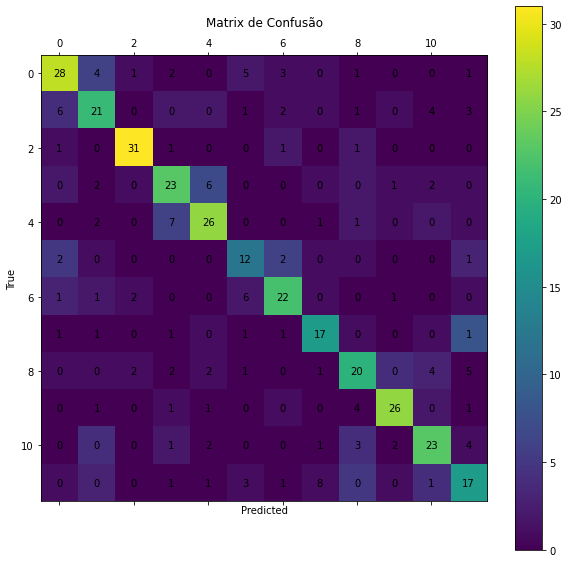
\includegraphics[width=18em]{experiments/lenet5_noaug_32/confusion_matrix.png}
  \caption{Matrix de Confusão}
  \label{fig:experiment_lenet5_noaug_32_confusion_matrix}
\end{figure}

\begin{table}[!htb]
  \centering
  \begin{tabular}{|c|c|c|c|}
    \hline
    \textbf{Experimento} & \textbf{Loss} & \textbf{Acurácia} & \textbf{Tempo de Execução (s)} \\ \hline
    lenet5\_noaug\_32    & 1.00          & 0.66              & 5.78                           \\ \hline
  \end{tabular}
  \caption{Resultados Obtidos (lenet5\_noaug\_32)}
  \label{tab:experiment_lenet5_noaug_32_reults}
\end{table}

\newpage

\subsection{lenet5\_noaug\_64}

Após a execução deste experimento, obteve-se o gráfico de evolução da acurácia (Figura \ref{fig:experiment_lenet5_noaug_64_accuracy}), o gráfico de perda durante o treinamento (Figura \ref{fig:experiment_lenet5_noaug_64_loss}) e a representação da matriz de confusão (Figura \ref{fig:experiment_lenet5_noaug_64_confusion_matrix}). A Tabela \ref{tab:experiment_lenet5_noaug_64_reults} sumariza os resultados obtidos.

\begin{figure}[!htb]
  \begin{minipage}{.47\textwidth}
    \centering
    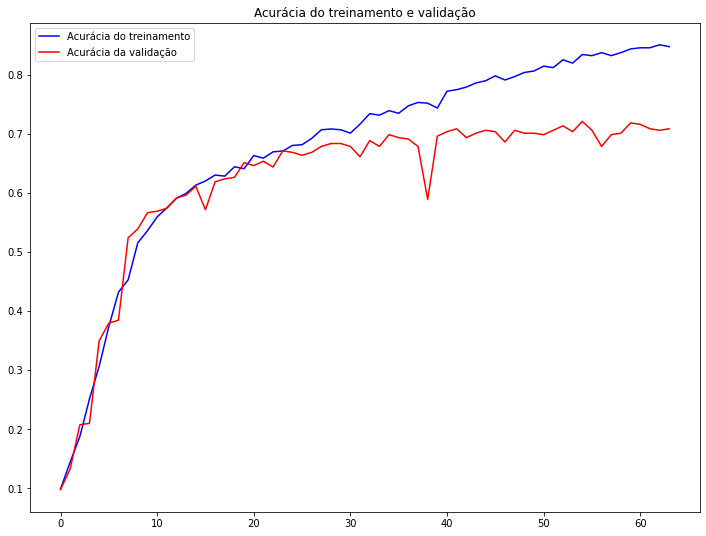
\includegraphics[width=1.1\linewidth]{experiments/lenet5_noaug_64/accuracy.png}
    \caption{Acurácia}\label{fig:experiment_lenet5_noaug_64_accuracy}
  \end{minipage}\hfill
  \begin{minipage}{.47\textwidth}
    \centering
    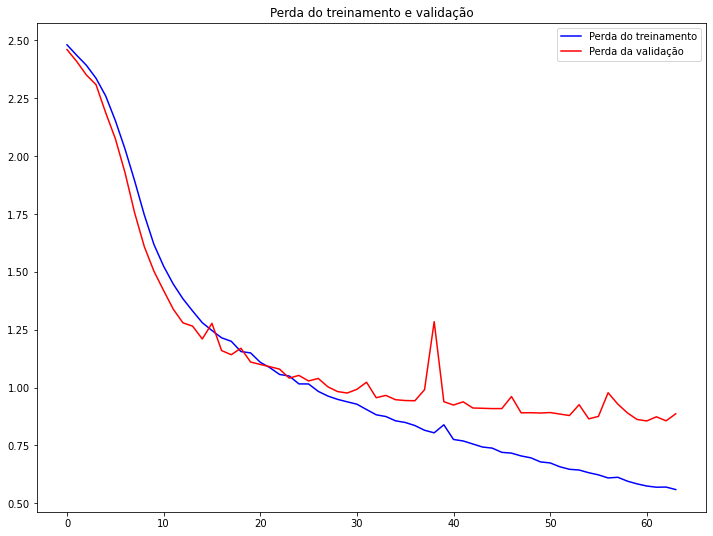
\includegraphics[width=1.1\linewidth]{experiments/lenet5_noaug_64/loss.png}
    \caption{Perda}\label{fig:experiment_lenet5_noaug_64_loss}
  \end{minipage}
\end{figure}

\begin{figure}[!htb]
  \centering
  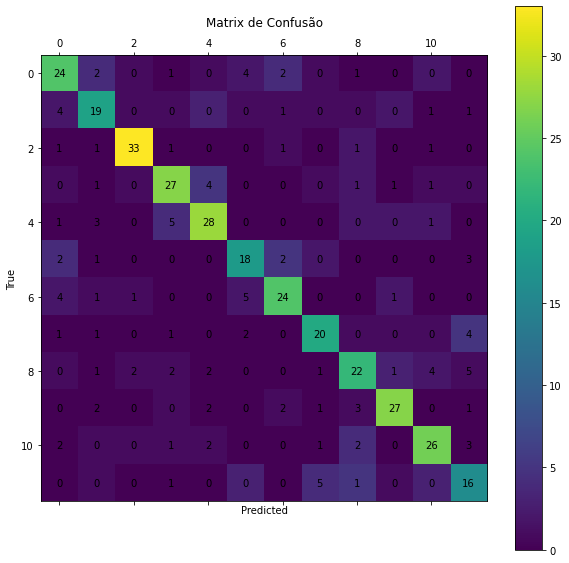
\includegraphics[width=18em]{experiments/lenet5_noaug_64/confusion_matrix.png}
  \caption{Matrix de Confusão}
  \label{fig:experiment_lenet5_noaug_64_confusion_matrix}
\end{figure}

\begin{table}[!htb]
  \centering
  \begin{tabular}{|c|c|c|c|}
    \hline
    \textbf{Experimento} & \textbf{Loss} & \textbf{Acurácia} & \textbf{Tempo de Execução (s)} \\ \hline
    lenet5\_noaug\_64    & 0.88          & 0.70              & 9.51                           \\ \hline
  \end{tabular}
  \caption{Resultados Obtidos (lenet5\_noaug\_64)}
  \label{tab:experiment_lenet5_noaug_64_reults}
\end{table}

\newpage

\subsection{lenet5\_noaug\_128}

Após a execução deste experimento, obteve-se o gráfico de evolução da acurácia (Figura \ref{fig:experiment_lenet5_noaug_128_accuracy}), o gráfico de perda durante o treinamento (Figura \ref{fig:experiment_lenet5_noaug_128_loss}) e a representação da matriz de confusão (Figura \ref{fig:experiment_lenet5_noaug_128_confusion_matrix}). A Tabela \ref{tab:experiment_lenet5_noaug_128_reults} sumariza os resultados obtidos.

\begin{figure}[!htb]
  \begin{minipage}{.47\textwidth}
    \centering
    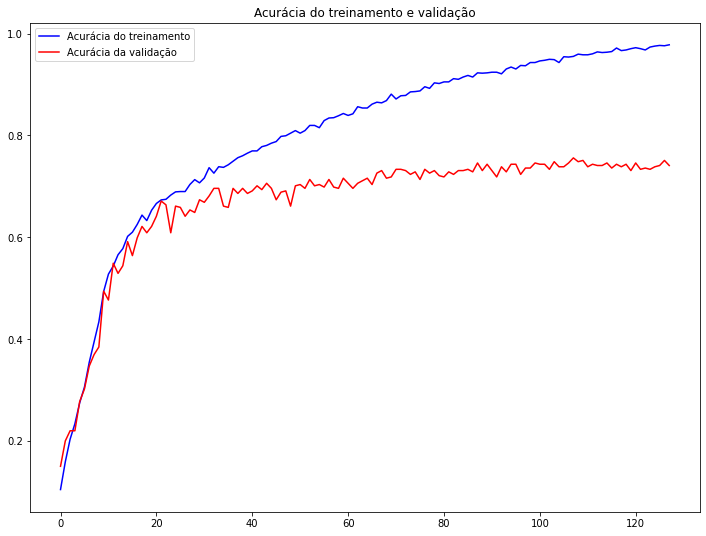
\includegraphics[width=1.1\linewidth]{experiments/lenet5_noaug_128/accuracy.png}
    \caption{Acurácia}\label{fig:experiment_lenet5_noaug_128_accuracy}
  \end{minipage}\hfill
  \begin{minipage}{.47\textwidth}
    \centering
    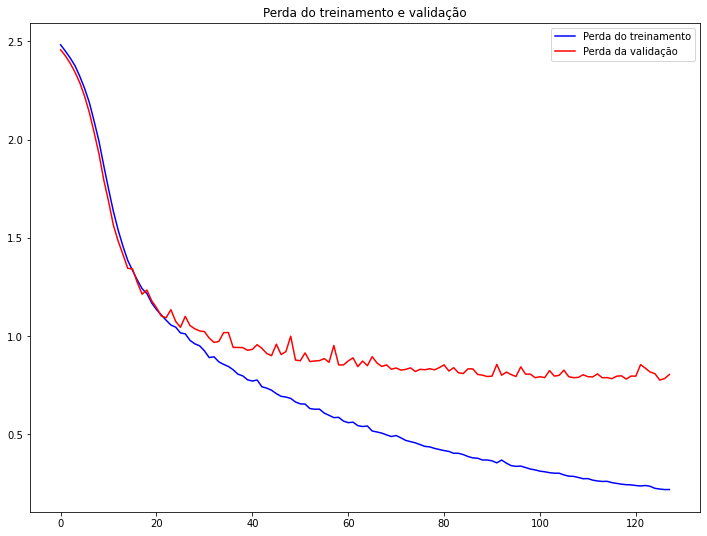
\includegraphics[width=1.1\linewidth]{experiments/lenet5_noaug_128/loss.png}
    \caption{Perda}\label{fig:experiment_lenet5_noaug_128_loss}
  \end{minipage}
\end{figure}

\begin{figure}[!htb]
  \centering
  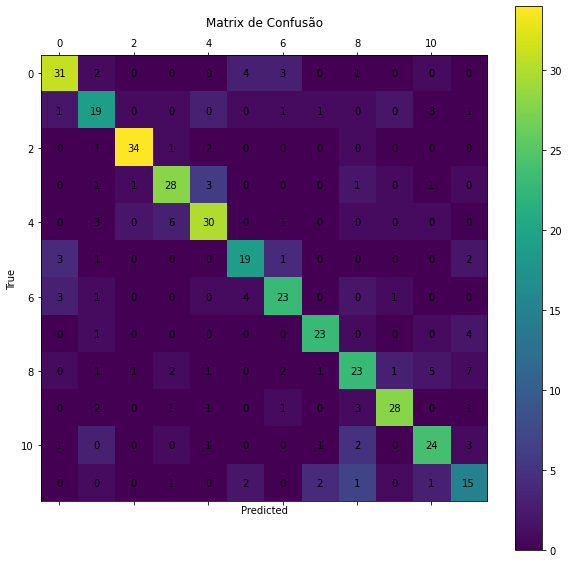
\includegraphics[width=18em]{experiments/lenet5_noaug_128/confusion_matrix.png}
  \caption{Matrix de Confusão}
  \label{fig:experiment_lenet5_noaug_128_confusion_matrix}
\end{figure}

\begin{table}[!htb]
  \centering
  \begin{tabular}{|c|c|c|c|}
    \hline
    \textbf{Experimento} & \textbf{Loss} & \textbf{Acurácia} & \textbf{Tempo de Execução (s)} \\ \hline
    lenet5\_noaug\_128   & 0.80          & 0.74              & 16.44                          \\ \hline
  \end{tabular}
  \caption{Resultados Obtidos (lenet5\_noaug\_128)}
  \label{tab:experiment_lenet5_noaug_128_reults}
\end{table}

\newpage

\subsection{default\_noaug\_32}

Após a execução deste experimento, obteve-se o gráfico de evolução da acurácia (Figura \ref{fig:experiment_default_noaug_32_accuracy}), o gráfico de perda durante o treinamento (Figura \ref{fig:experiment_default_noaug_32_loss}) e a representação da matriz de confusão (Figura \ref{fig:experiment_default_noaug_32_confusion_matrix}). A Tabela \ref{tab:experiment_default_noaug_32_reults} sumariza os resultados obtidos.

\begin{figure}[!htb]
  \begin{minipage}{.47\textwidth}
    \centering
    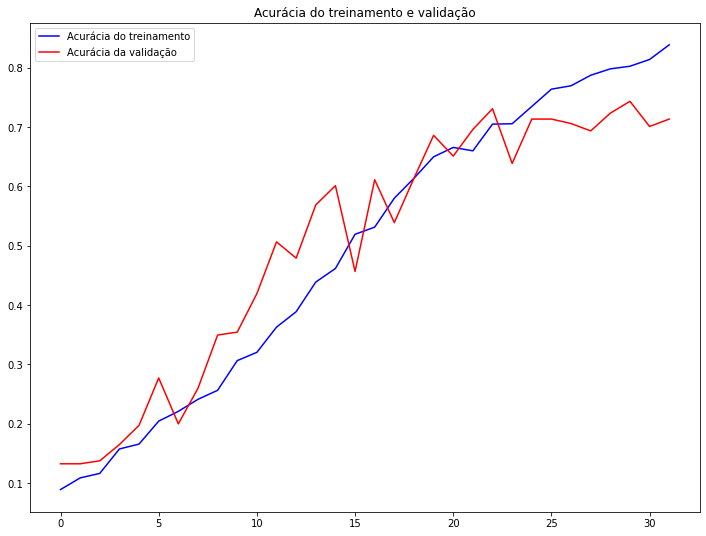
\includegraphics[width=1.1\linewidth]{experiments/default_noaug_32/accuracy.png}
    \caption{Acurácia}\label{fig:experiment_default_noaug_32_accuracy}
  \end{minipage}\hfill
  \begin{minipage}{.47\textwidth}
    \centering
    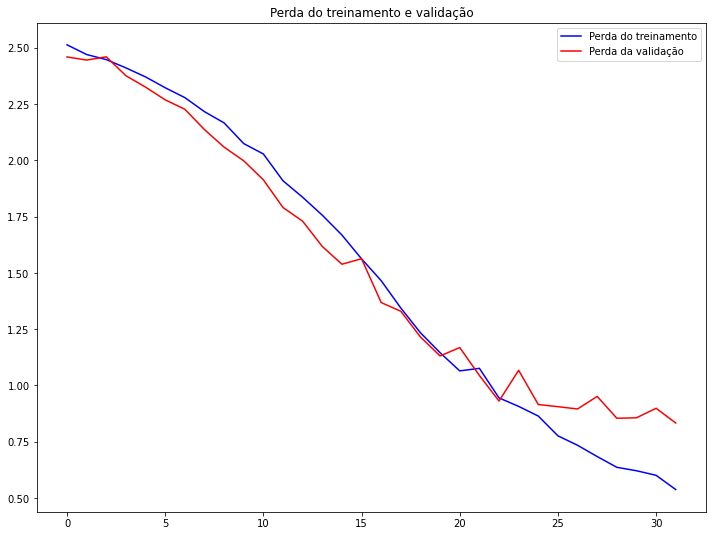
\includegraphics[width=1.1\linewidth]{experiments/default_noaug_32/loss.png}
    \caption{Perda}\label{fig:experiment_default_noaug_32_loss}
  \end{minipage}
\end{figure}

\begin{figure}[!htb]
  \centering
  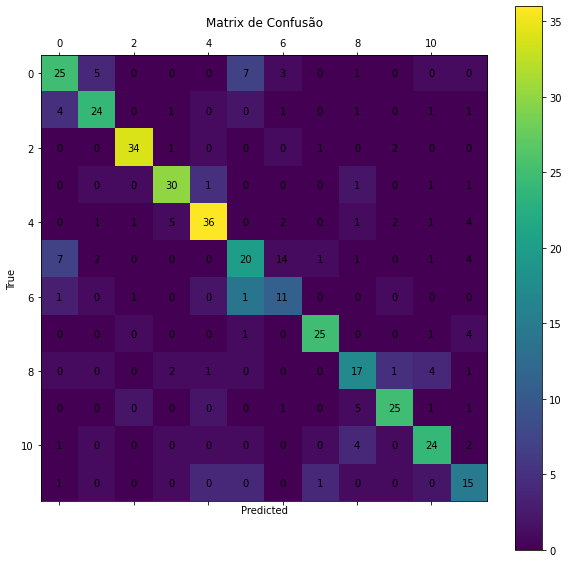
\includegraphics[width=18em]{experiments/default_noaug_32/confusion_matrix.png}
  \caption{Matrix de Confusão}
  \label{fig:experiment_default_noaug_32_confusion_matrix}
\end{figure}

\begin{table}[!htb]
  \centering
  \begin{tabular}{|c|c|c|c|}
    \hline
    \textbf{Experimento} & \textbf{Loss} & \textbf{Acurácia} & \textbf{Tempo de Execução (s)} \\ \hline
    default\_noaug\_32   & 0.83          & 0.71              & 12.37                          \\ \hline
  \end{tabular}
  \caption{Resultados Obtidos (default\_noaug\_32)}
  \label{tab:experiment_default_noaug_32_reults}
\end{table}

\newpage

\subsection{default\_noaug\_64}

Após a execução deste experimento, obteve-se o gráfico de evolução da acurácia (Figura \ref{fig:experiment_default_noaug_64_accuracy}), o gráfico de perda durante o treinamento (Figura \ref{fig:experiment_default_noaug_64_loss}) e a representação da matrix de confusão (Figura \ref{fig:experiment_default_noaug_64_confusion_matrix}). A Tabela \ref{tab:experiment_default_noaug_64_reults} sumariza os resultados obtidos.

\begin{figure}[!htb]
  \begin{minipage}{.47\textwidth}
    \centering
    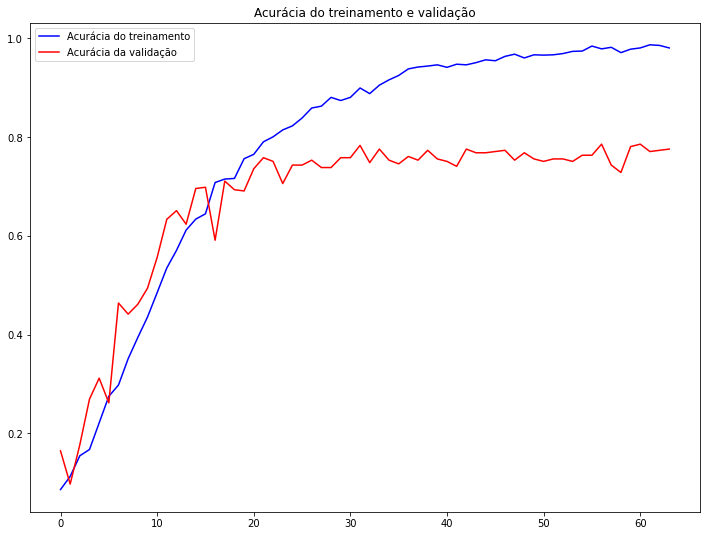
\includegraphics[width=1.1\linewidth]{experiments/default_noaug_64/accuracy.png}
    \caption{Acurácia}\label{fig:experiment_default_noaug_64_accuracy}
  \end{minipage}\hfill
  \begin{minipage}{.47\textwidth}
    \centering
    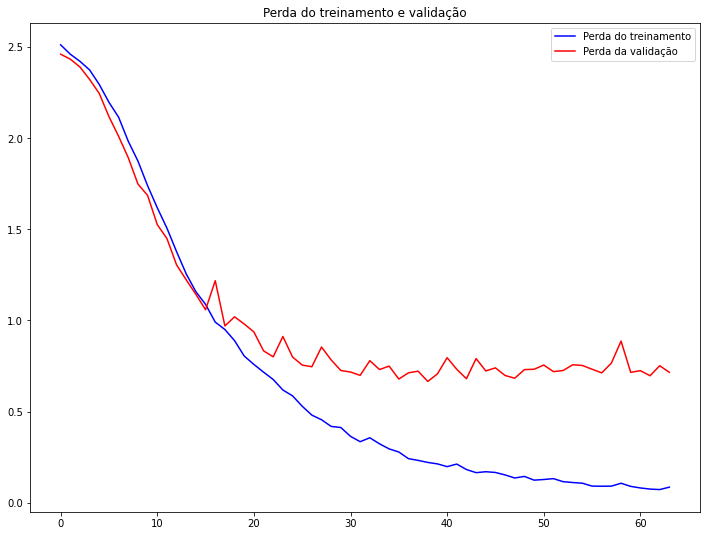
\includegraphics[width=1.1\linewidth]{experiments/default_noaug_64/loss.png}
    \caption{Perda}\label{fig:experiment_default_noaug_64_loss}
  \end{minipage}
\end{figure}

\begin{figure}[!htb]
  \centering
  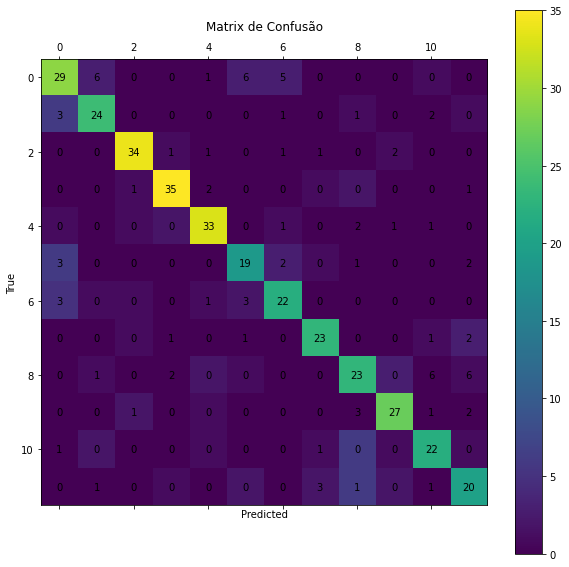
\includegraphics[width=18em]{experiments/default_noaug_64/confusion_matrix.png}
  \caption{Matrix de Confusão}
  \label{fig:experiment_default_noaug_64_confusion_matrix}
\end{figure}

\begin{table}[!htb]
  \centering
  \begin{tabular}{|c|c|c|c|}
    \hline
    \textbf{Experimento} & \textbf{Loss} & \textbf{Acurácia} & \textbf{Tempo de Execução (s)} \\ \hline
    default\_noaug\_64   & 0.71          & 0.77              & 21.38                          \\ \hline
  \end{tabular}
  \caption{Resultados Obtidos (default\_noaug\_64)}
  \label{tab:experiment_default_noaug_64_reults}
\end{table}

\newpage

\subsection{default\_noaug\_128}

Após a execução deste experimento, obteve-se o gráfico de evolução da acurácia (Figura \ref{fig:experiment_default_noaug_128_accuracy}), o gráfico de perda durante o treinamento (Figura \ref{fig:experiment_default_noaug_128_loss}) e a representação da matriz de confusão (Figura \ref{fig:experiment_default_noaug_128_confusion_matrix}). A Tabela \ref{tab:experiment_default_noaug_128_reults} sumariza os resultados obtidos.

\begin{figure}[!htb]
  \begin{minipage}{.47\textwidth}
    \centering
    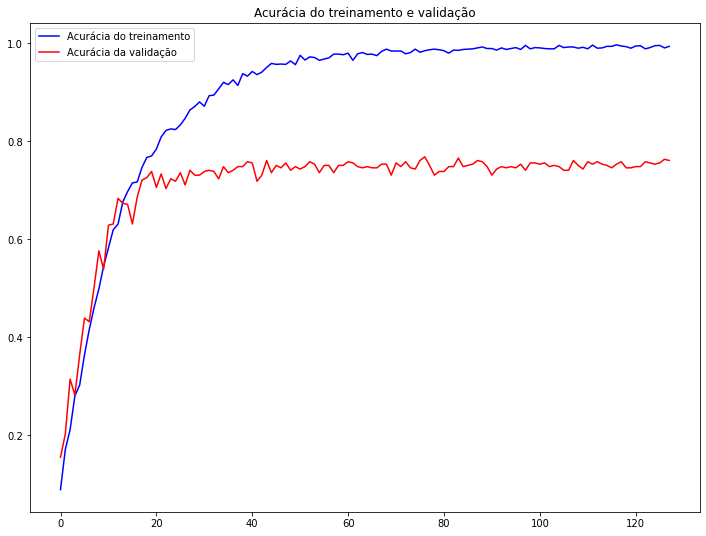
\includegraphics[width=1.1\linewidth]{experiments/default_noaug_128/accuracy.png}
    \caption{Acurácia}\label{fig:experiment_default_noaug_128_accuracy}
  \end{minipage}\hfill
  \begin{minipage}{.47\textwidth}
    \centering
    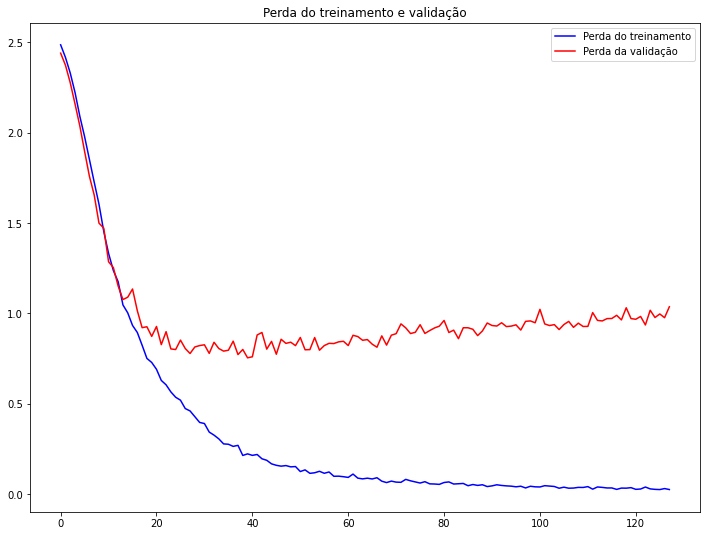
\includegraphics[width=1.1\linewidth]{experiments/default_noaug_128/loss.png}
    \caption{Perda}\label{fig:experiment_default_noaug_128_loss}
  \end{minipage}
\end{figure}

\begin{figure}[!htb]
  \centering
  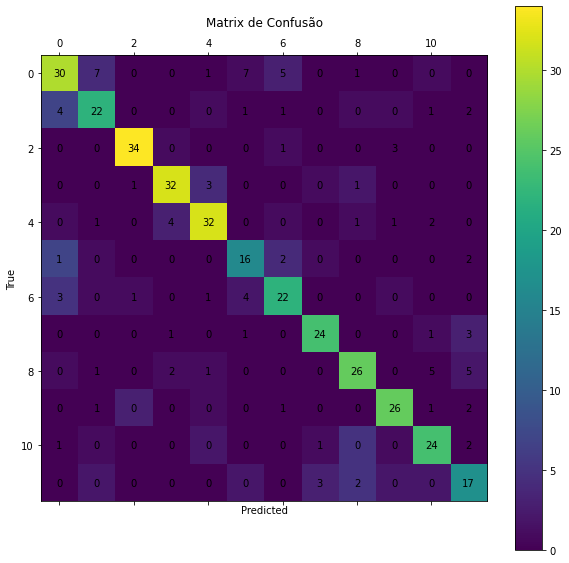
\includegraphics[width=18em]{experiments/default_noaug_128/confusion_matrix.png}
  \caption{Matrix de Confusão}
  \label{fig:experiment_default_noaug_128_confusion_matrix}
\end{figure}

\begin{table}[!htb]
  \centering
  \begin{tabular}{|c|c|c|c|}
    \hline
    \textbf{Experimento} & \textbf{Loss} & \textbf{Acurácia} & \textbf{Tempo de Execução (s)} \\ \hline
    default\_noaug\_128  & 1.03          & 0.76              & 40.14                          \\ \hline
  \end{tabular}
  \caption{Resultados Obtidos (default\_noaug\_128)}
  \label{tab:experiment_default_noaug_128_reults}
\end{table}

\newpage

\section{Implementação de Data Augmentation}

Neste ponto do experimento, foram implementadas técnicas para a realização de \textit{data augmentation}. Para isso, foram implementadas funções específicas para a realização de pequenas variações nas imagens da base de treinamento original. O Código \ref{code:data_augmentation} mostra quais foram as funções utilizadas para a realização destas transformações.

\begin{lstlisting}[caption={Funções de Transformação das Imagens},captionpos=b,frame=single,label={code:data_augmentation}]
flip_rotation_brightness_zoom(path, zoom=[0.5, 1.0], brightness=[0.2, 1.0], rotation=90, flip_horizontal=False,
flip_vertical=False, subdir="zoom")

random_zoom(path, zoom=[0.5, 1.0], subdir="zoom")

random_brightness(path, brightness=[0.2, 1.0], subdir="brightness")

random_rotation(path, rotation=90, subdir="rotation")

horizontal_vertical_flip(path, flip_horizontal=False, flip_vertical=False, subdir="flip")

orizontal_vertical_shift(path, size=0.5, bool_width=True, subdir="shift")
\end{lstlisting}

A função \textbf{flip\_rotation\_brightness\_zoom} realiza transformações de rotação, brilho e zoom na imagem. A função \textbf{random\_zoom} realiza a transformação de zoom da imagem. A função \textbf{random\_brightness} realiza a transformação de brilho da imagem. A função \textbf{random\_rotation} realiza a transformação de rotacão da imagem. A função \textbf{horizontal\_vertical\_flip} realiza a transformação de flip vertical. A função \textbf{horizontal\_vertical\_shift} realiza a transformação de shift. Todas as funções possuem parâmetros.

Para imagem da base de treinamento foram realizadas as operações descritas no Código \ref{code:data_augmentation_executed}.

\newpage

\begin{lstlisting}[caption={Funções de Augmentation Executadas},captionpos=b,frame=single,label={code:data_augmentation_executed}]
horizontal_vertical_flip(image_path, flip_horizontal=True, flip_vertical=False)
horizontal_vertical_flip(image_path, flip_horizontal=False, flip_vertical=True)
horizontal_vertical_flip(image_path, flip_horizontal=True, flip_vertical=True)
horizontal_vertical_flip(image_path, flip_horizontal=False, flip_vertical=False)
horizontal_vertical_shift(image_path, bool_width=True)
horizontal_vertical_shift(image_path, bool_width=False)
random_rotation(image_path, rotation=10)
random_rotation(image_path, rotation=20)
random_rotation(image_path, rotation=30)
random_rotation(image_path, rotation=45)
random_brightness(image_path)
random_brightness(image_path, brightness=[0.1, 0.2])
random_brightness(image_path, brightness=[0.3, 0.4])
random_brightness(image_path, brightness=[0.4, 0.5])
random_zoom(image_path)
random_zoom(image_path, zoom=[0.1, 0.5])
random_zoom(image_path, zoom=[0.1, 0.2])
random_zoom(image_path, zoom=[0.1, 0.3])
flip_rotation_brightness_zoom(image_path, rotation=30)
flip_rotation_brightness_zoom(image_path, zoom=[0.1, 0.5], brightness=[0.1, 0.5])
flip_rotation_brightness_zoom(image_path, zoom=[0.1, 0.5], brightness=[0.1, 0.5])
flip_rotation_brightness_zoom(image_path, zoom=[0.1, 0.5], brightness=[0.1, 0.5], rotation=30)
flip_rotation_brightness_zoom(image_path, zoom=[0.1, 0.5], brightness=[0.1, 0.5], rotation=30)
flip_rotation_brightness_zoom(image_path, zoom=[0.1, 0.5], brightness=[0.1, 0.5], rotation=30)
flip_rotation_brightness_zoom(image_path, zoom=[0.1, 0.8], brightness=[0.1, 0.8], rotation=45)
flip_rotation_brightness_zoom(image_path, zoom=[0.1, 0.8], brightness=[0.1, 0.8], rotation=45)
flip_rotation_brightness_zoom(image_path, zoom=[0.1, 0.2], brightness=[0.1, 0.2], rotation=30)
flip_rotation_brightness_zoom(image_path, zoom=[0.1, 0.2], brightness=[0.1, 0.2], rotation=45)
flip_rotation_brightness_zoom(image_path, zoom=[0.9, 1], brightness=[0.9, 1], rotation=30)
flip_rotation_brightness_zoom(image_path, zoom=[0.9, 1], brightness=[0.9, 1], rotation=45)
  \end{lstlisting}

A base inicial de treinamento, é composta por \textbf{1578} imagens. Após execução do \textit{script}, obteve-se o total de \textbf{27558} imagens.

\newpage

\subsection{lenet5\_aug\_32}

Após a execução deste experimento, obteve-se o gráfico de evolução da acurácia (Figura \ref{fig:experiment_lenet5_aug_32_accuracy}), o gráfico de perda durante o treinamento (Figura \ref{fig:experiment_lenet5_aug_32_loss}) e a representação da matriz de confusão (Figura \ref{fig:experiment_lenet5_aug_32_confusion_matrix}). A Tabela \ref{tab:experiment_lenet5_aug_32_reults} sumariza os resultados obtidos.

\begin{figure}[!htb]
  \begin{minipage}{.47\textwidth}
    \centering
    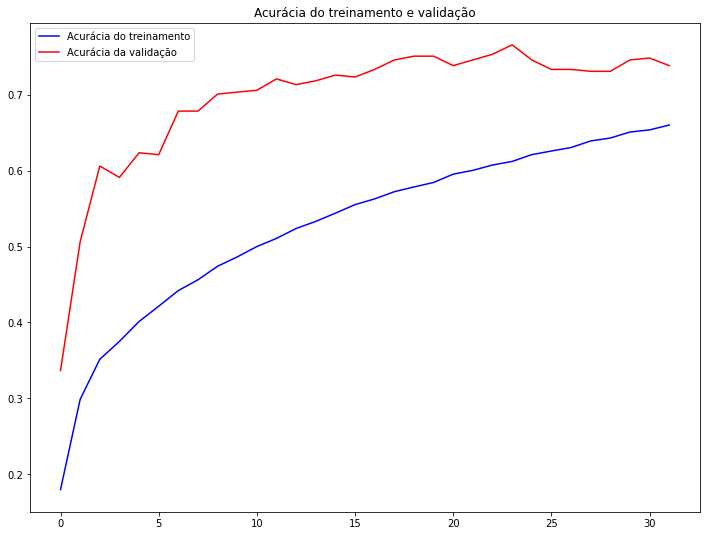
\includegraphics[width=1.1\linewidth]{experiments/lenet5_aug_32/accuracy.png}
    \caption{Acurácia}\label{fig:experiment_lenet5_aug_32_accuracy}
  \end{minipage}\hfill
  \begin{minipage}{.47\textwidth}
    \centering
    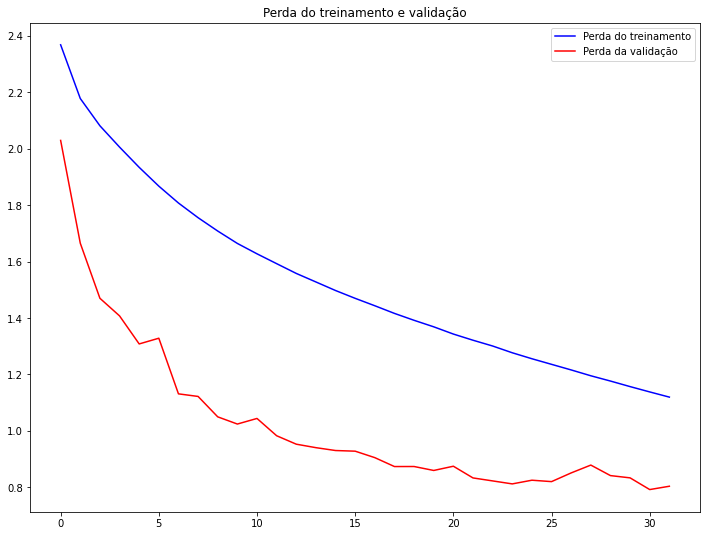
\includegraphics[width=1.1\linewidth]{experiments/lenet5_aug_32/loss.png}
    \caption{Perda}\label{fig:experiment_lenet5_aug_32_loss}
  \end{minipage}
\end{figure}

\begin{figure}[!htb]
  \centering
  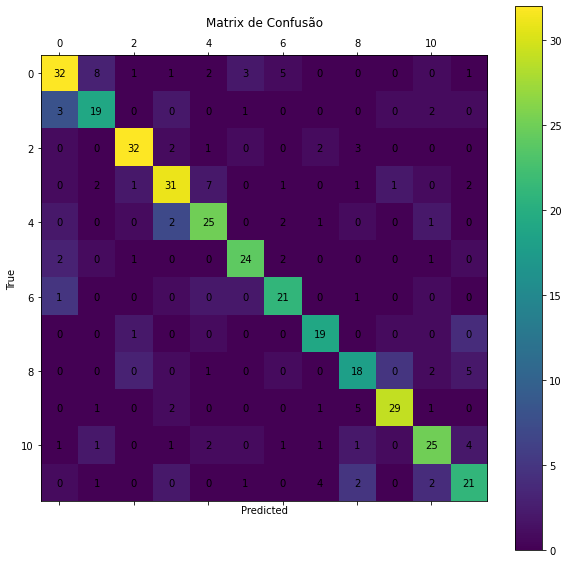
\includegraphics[width=18em]{experiments/lenet5_aug_32/confusion_matrix.png}
  \caption{Matrix de Confusão}
  \label{fig:experiment_lenet5_aug_32_confusion_matrix}
\end{figure}

\begin{table}[!htb]
  \centering
  \begin{tabular}{|c|c|c|c|}
    \hline
    \textbf{Experimento} & \textbf{Loss} & \textbf{Acurácia} & \textbf{Tempo de Execução (s)} \\ \hline
    lenet5\_aug\_32      & 0.80          & 0.73              & 63.91                          \\ \hline
  \end{tabular}
  \caption{Resultados Obtidos (lenet5\_aug\_32)}
  \label{tab:experiment_lenet5_aug_32_reults}
\end{table}

\newpage

\subsection{lenet5\_aug\_64}

Após a execução deste experimento, obteve-se o gráfico de evolução da acurácia (Figura \ref{fig:experiment_lenet5_aug_64_accuracy}), o gráfico de perda durante o treinamento (Figura \ref{fig:experiment_lenet5_aug_64_loss}) e a representação da matriz de confusão (Figura \ref{fig:experiment_lenet5_aug_64_confusion_matrix}). A Tabela \ref{tab:experiment_lenet5_aug_64_reults} sumariza os resultados obtidos.

\begin{figure}[!htb]
  \begin{minipage}{.47\textwidth}
    \centering
    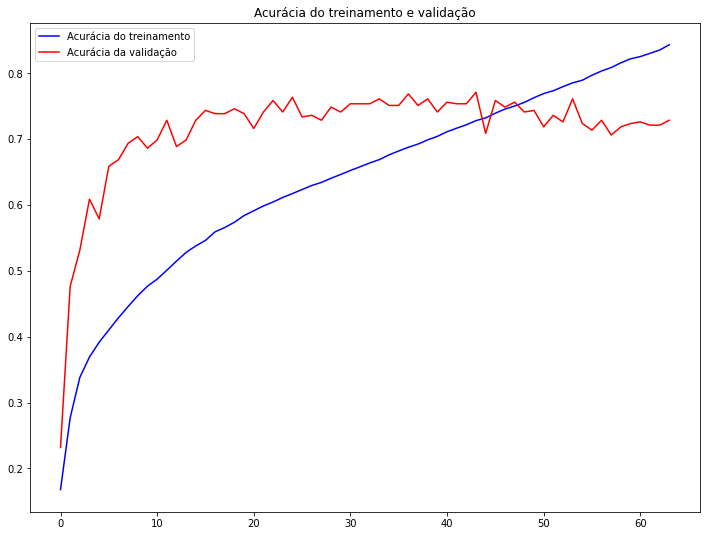
\includegraphics[width=1.1\linewidth]{experiments/lenet5_aug_64/accuracy.png}
    \caption{Acurácia}\label{fig:experiment_lenet5_aug_64_accuracy}
  \end{minipage}\hfill
  \begin{minipage}{.47\textwidth}
    \centering
    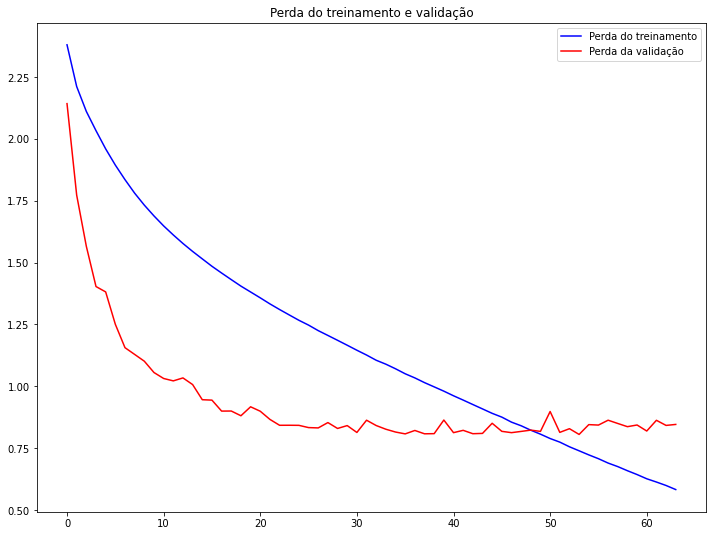
\includegraphics[width=1.1\linewidth]{experiments/lenet5_aug_64/loss.png}
    \caption{Perda}\label{fig:experiment_lenet5_aug_64_loss}
  \end{minipage}
\end{figure}

\begin{figure}[!htb]
  \centering
  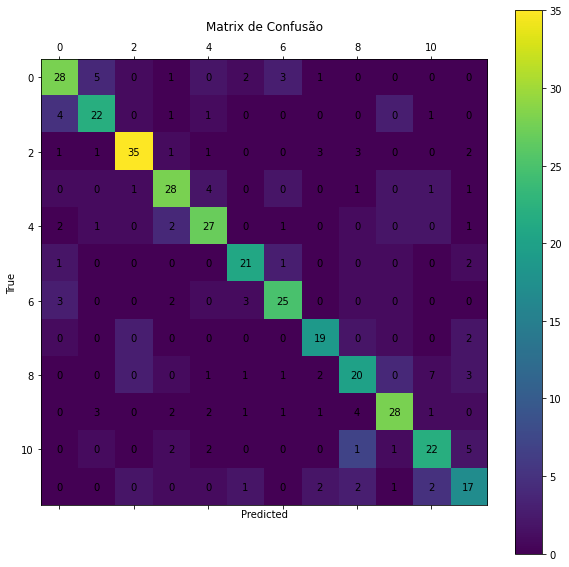
\includegraphics[width=18em]{experiments/lenet5_aug_64/confusion_matrix.png}
  \caption{Matrix de Confusão}
  \label{fig:experiment_lenet5_aug_64_confusion_matrix}
\end{figure}

\begin{table}[!htb]
  \centering
  \begin{tabular}{|c|c|c|c|}
    \hline
    \textbf{Experimento} & \textbf{Loss} & \textbf{Acurácia} & \textbf{Tempo de Execução (s)} \\ \hline
    lenet5\_aug\_64      & 0.84          & 0.72              & 105.89                         \\ \hline
  \end{tabular}
  \caption{Resultados Obtidos (lenet5\_aug\_64)}
  \label{tab:experiment_lenet5_aug_64_reults}
\end{table}

\newpage

\subsection{lenet5\_aug\_128}

Após a execução deste experimento, obteve-se o gráfico de evolução da acurácia (Figura \ref{fig:experiment_lenet5_aug_128_accuracy}), o gráfico de perda durante o treinamento (Figura \ref{fig:experiment_lenet5_aug_128_loss}) e a representação da matriz de confusão (Figura \ref{fig:experiment_lenet5_aug_128_confusion_matrix}). A Tabela \ref{tab:experiment_lenet5_aug_128_reults} sumariza os resultados obtidos.

\begin{figure}[!htb]
  \begin{minipage}{.47\textwidth}
    \centering
    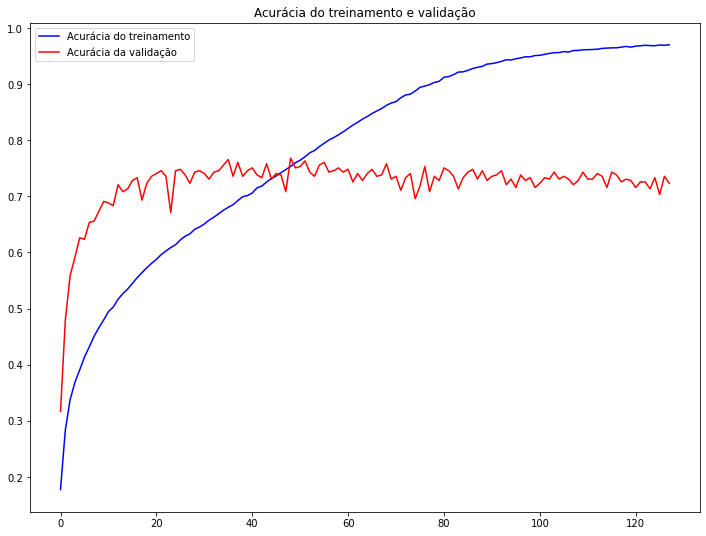
\includegraphics[width=1.1\linewidth]{experiments/lenet5_aug_128/accuracy.png}
    \caption{Acurácia}\label{fig:experiment_lenet5_aug_128_accuracy}
  \end{minipage}\hfill
  \begin{minipage}{.47\textwidth}
    \centering
    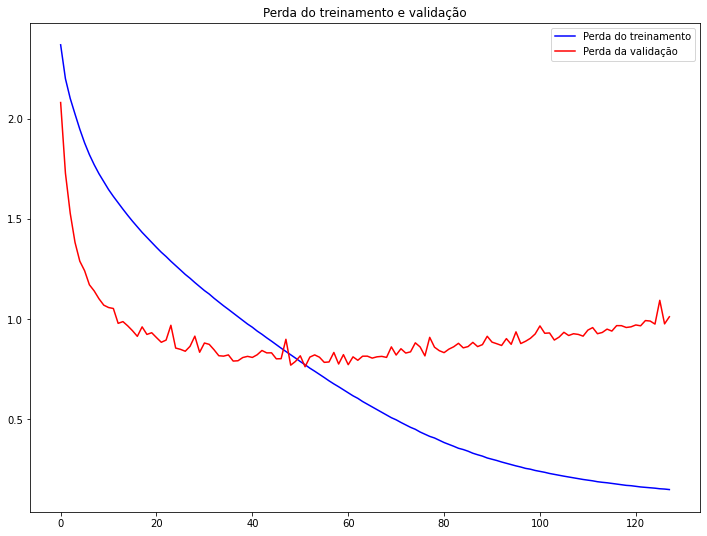
\includegraphics[width=1.1\linewidth]{experiments/lenet5_aug_128/loss.png}
    \caption{Perda}\label{fig:experiment_lenet5_aug_128_loss}
  \end{minipage}
\end{figure}

\begin{figure}[!htb]
  \centering
  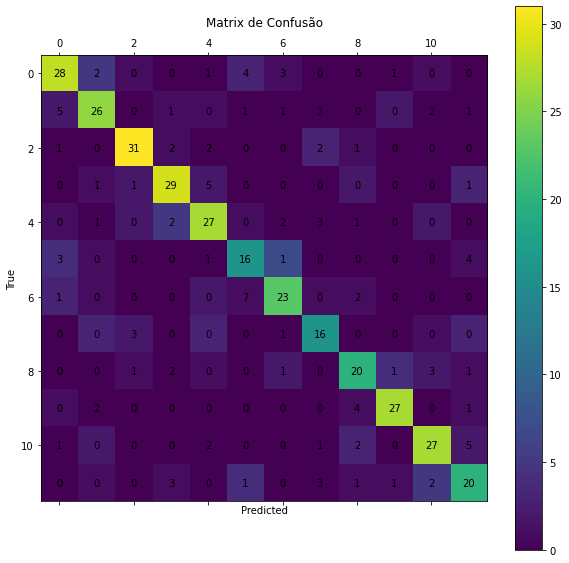
\includegraphics[width=18em]{experiments/lenet5_aug_128/confusion_matrix.png}
  \caption{Matrix de Confusão}
  \label{fig:experiment_lenet5_aug_128_confusion_matrix}
\end{figure}

\begin{table}[!htb]
  \centering
  \begin{tabular}{|c|c|c|c|}
    \hline
    \textbf{Experimento} & \textbf{Loss} & \textbf{Acurácia} & \textbf{Tempo de Execução (s)} \\ \hline
    lenet5\_aug\_128     & 1.01          & 0.72              & 193.93                         \\ \hline
  \end{tabular}
  \caption{Resultados Obtidos (lenet5\_aug\_128)}
  \label{tab:experiment_lenet5_aug_128_reults}
\end{table}

\subsection{custom\_aug\_32}

Após a execução deste experimento, obteve-se o gráfico de evolução da acurácia (Figura \ref{fig:experiment_default_aug_32_accuracy}), o gráfico de perda durante o treinamento (Figura \ref{fig:experiment_default_aug_32_loss}) e a representação da matriz de confusão (Figura \ref{fig:experiment_default_aug_32_confusion_matrix}). A Tabela \ref{tab:experiment_default_aug_32_reults} sumariza os resultados obtidos.

\begin{figure}[!htb]
  \begin{minipage}{.47\textwidth}
    \centering
    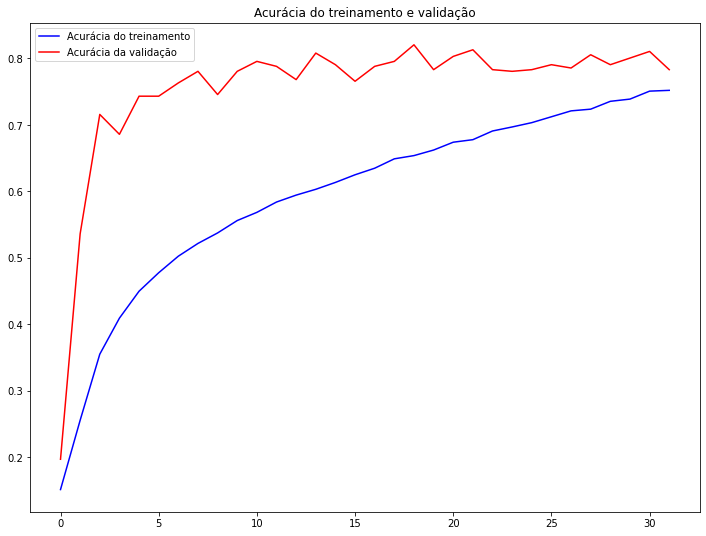
\includegraphics[width=1.1\linewidth]{experiments/default_aug_32/accuracy.png}
    \caption{Acurácia}\label{fig:experiment_default_aug_32_accuracy}
  \end{minipage}\hfill
  \begin{minipage}{.47\textwidth}
    \centering
    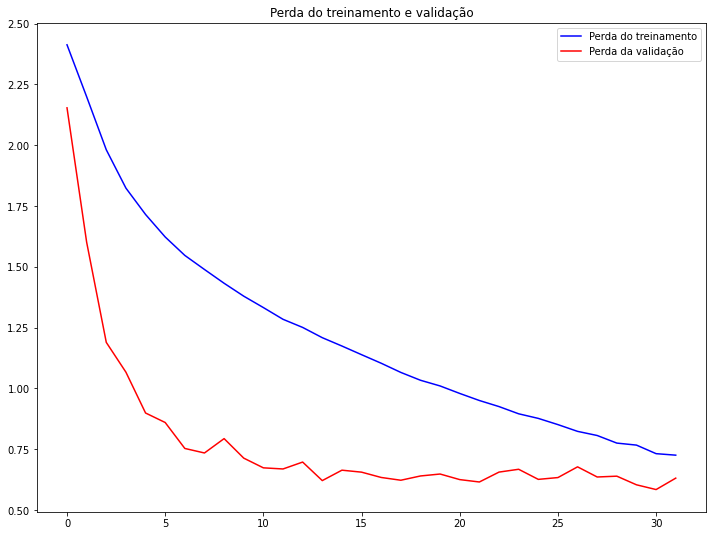
\includegraphics[width=1.1\linewidth]{experiments/default_aug_32/loss.png}
    \caption{Perda}\label{fig:experiment_default_aug_32_loss}
  \end{minipage}
\end{figure}

\begin{figure}[!htb]
  \centering
  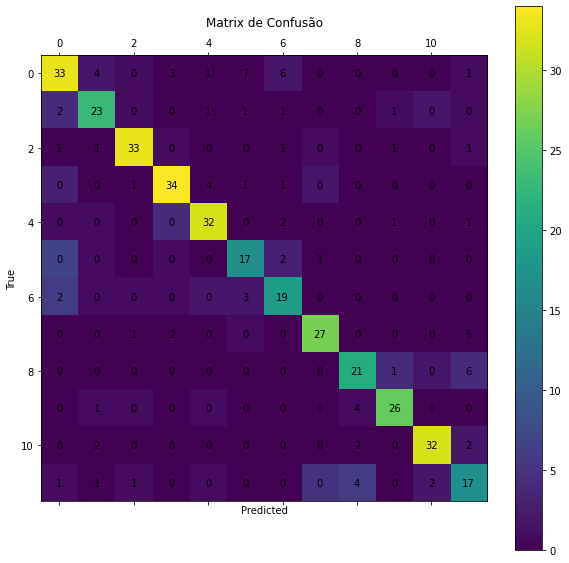
\includegraphics[width=18em]{experiments/default_aug_32/confusion_matrix.png}
  \caption{Matrix de Confusão}
  \label{fig:experiment_default_aug_32_confusion_matrix}
\end{figure}

\begin{table}[!htb]
  \centering
  \begin{tabular}{|c|c|c|c|}
    \hline
    \textbf{Experimento} & \textbf{Loss} & \textbf{Acurácia} & \textbf{Tempo de Execução (s)} \\ \hline
    default\_aug\_32     & 0.63          & 0.78              & 159.49                         \\ \hline
  \end{tabular}
  \caption{Resultados Obtidos (custom\_aug\_32)}
  \label{tab:experiment_default_aug_32_reults}
\end{table}

\newpage

\subsection{custom\_aug\_64}

Após a execução deste experimento, obteve-se o gráfico de evolução da acurácia (Figura \ref{fig:experiment_default_aug_64_accuracy}), o gráfico de perda durante o treinamento (Figura \ref{fig:experiment_default_aug_64_loss}) e a representação da matriz de confusão (Figura \ref{fig:experiment_default_aug_64_confusion_matrix}). A Tabela \ref{tab:experiment_default_aug_64_reults} sumariza os resultados obtidos.

\begin{figure}[!htb]
  \begin{minipage}{.47\textwidth}
    \centering
    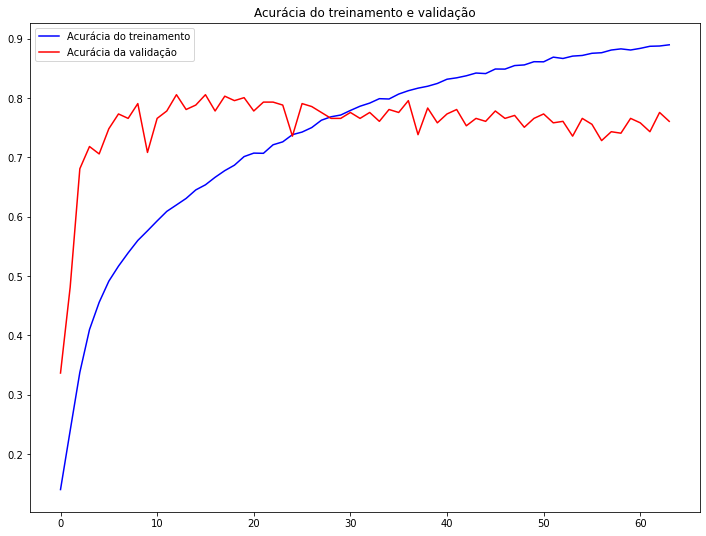
\includegraphics[width=1.1\linewidth]{experiments/default_aug_64/accuracy.png}
    \caption{Acurácia}\label{fig:experiment_default_aug_64_accuracy}
  \end{minipage}\hfill
  \begin{minipage}{.47\textwidth}
    \centering
    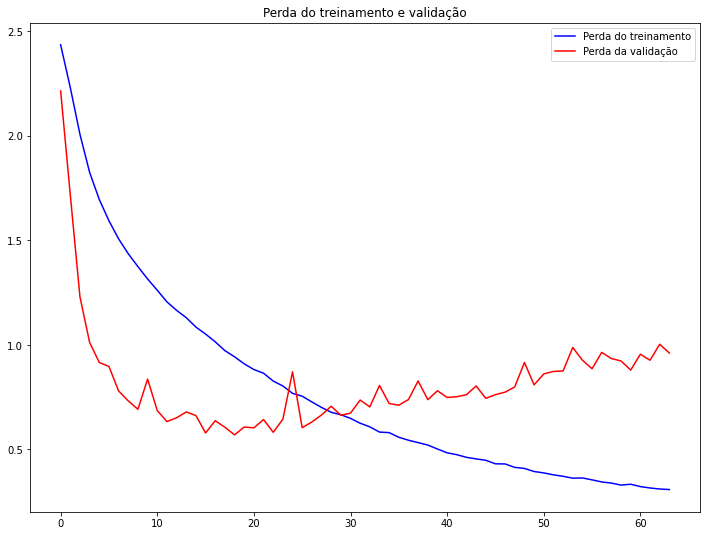
\includegraphics[width=1.1\linewidth]{experiments/default_aug_64/loss.png}
    \caption{Perda}\label{fig:experiment_default_aug_64_loss}
  \end{minipage}
\end{figure}

\begin{figure}[!htb]
  \centering
  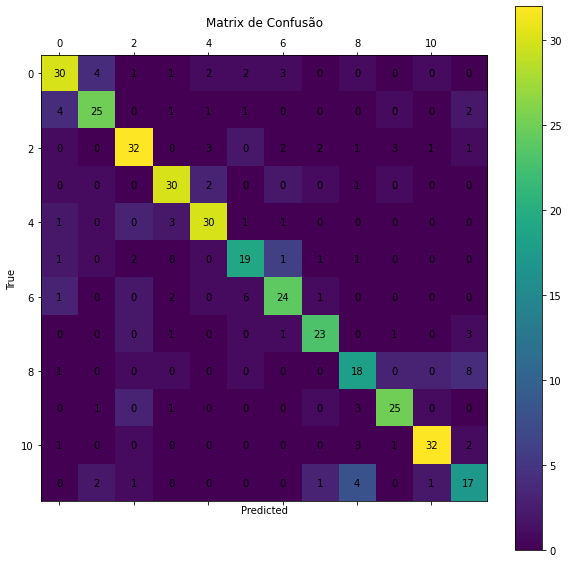
\includegraphics[width=18em]{experiments/default_aug_64/confusion_matrix.png}
  \caption{Matrix de Confusão}
  \label{fig:experiment_default_aug_64_confusion_matrix}
\end{figure}

\begin{table}[!htb]
  \centering
  \begin{tabular}{|c|c|c|c|}
    \hline
    \textbf{Experimento} & \textbf{Loss} & \textbf{Acurácia} & \textbf{Tempo de Execução (s)} \\ \hline
    default\_aug\_64     & 0.96          & 0.76              & 297.53                         \\ \hline
  \end{tabular}
  \caption{Resultados Obtidos (custom\_aug\_64)}
  \label{tab:experiment_default_aug_64_reults}
\end{table}

\newpage

\subsection{custom\_aug\_128}

Após a execução deste experimento, obteve-se o gráfico de evolução da acurácia (Figura \ref{fig:experiment_lenet5_aug_128_accuracy}), o gráfico de perda durante o treinamento (Figura \ref{fig:experiment_lenet5_aug_128_loss}) e a representação da matriz de confusão (Figura \ref{fig:experiment_lenet5_aug_128_confusion_matrix}). A Tabela \ref{tab:experiment_lenet5_aug_128_reults} sumariza os resultados obtidos.

\begin{figure}[!htb]
  \begin{minipage}{.47\textwidth}
    \centering
    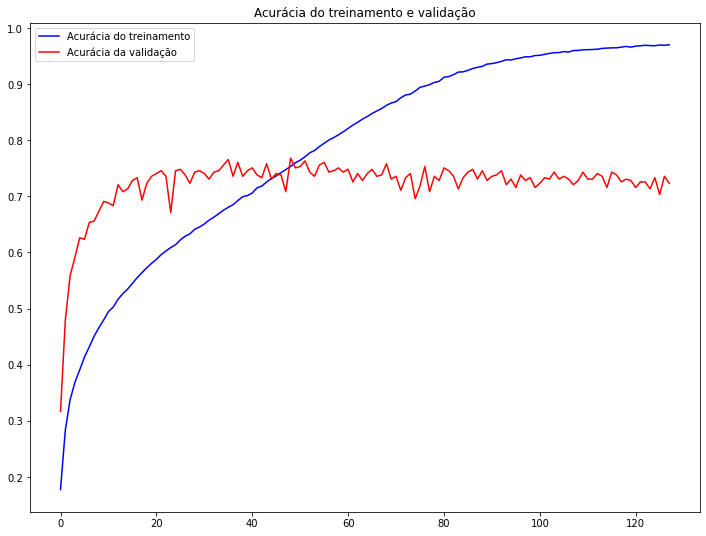
\includegraphics[width=1.1\linewidth]{experiments/lenet5_aug_128/accuracy.png}
    \caption{Acurácia}\label{fig:experiment_lenet5_aug_128_accuracy}
  \end{minipage}\hfill
  \begin{minipage}{.47\textwidth}
    \centering
    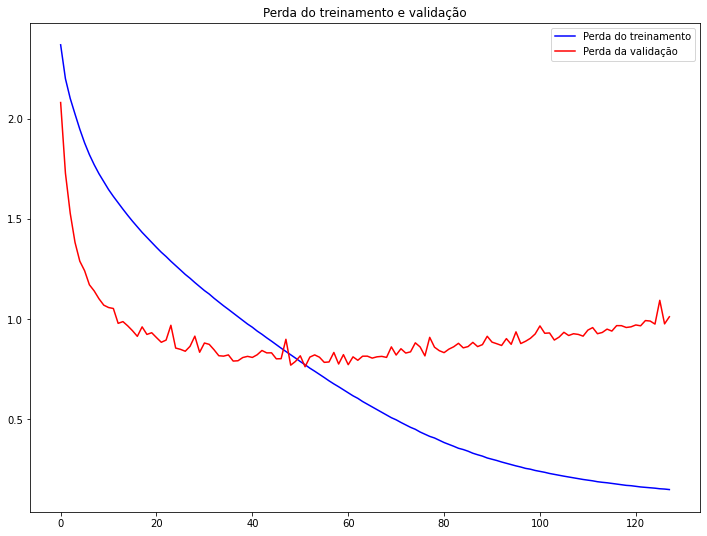
\includegraphics[width=1.1\linewidth]{experiments/lenet5_aug_128/loss.png}
    \caption{Perda}\label{fig:experiment_lenet5_aug_128_loss}
  \end{minipage}
\end{figure}

\begin{figure}[!htb]
  \centering
  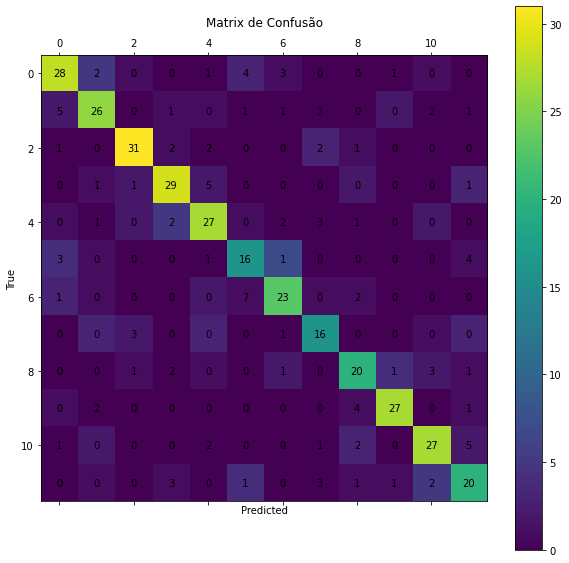
\includegraphics[width=18em]{experiments/lenet5_aug_128/confusion_matrix.png}
  \caption{Matrix de Confusão (custom\_aug\_64)}
  \label{fig:experiment_lenet5_aug_128_confusion_matrix}
\end{figure}

\begin{table}[!htb]
  \centering
  \begin{tabular}{|c|c|c|c|}
    \hline
    \textbf{Experimento} & \textbf{Loss} & \textbf{Acurácia} & \textbf{Tempo de Execução (s)} \\ \hline
    default\_aug\_128    & 1.26          & 0.76              & 557.75                         \\ \hline
  \end{tabular}
  \caption{Resultados Obtidos}
  \label{tab:experiment_lenet_aug_128_reults}
\end{table}

\section{Extração de Características}

Na sequência dos experimentos, utilizou-se um modelo pré-treinado da \textbf{ImageNet} para a extração das características das imagens, como demonstrado no Código \ref{code:imagenet_inception}.

\begin{lstlisting}[caption={ImageNet - InceptionV3},captionpos=b,frame=single,label={code:imagenet_inception}]
model = InceptionV3(weights='imagenet', include_top=False)
\end{lstlisting}

Como base de dados, utilizou-se inicialmente a base original sem data augmentation e na sequência, utilizou-se a base transformada pela técnica.

Foram realizados dois experimentos utilizando o classificador SVM, implementado pela biblioteca \textbf{Sklearn}. Criou-se arquivos de treinamento e teste para para a coleção de dados original e para a coleção com data augmentation.

As características foram extraídas das imagens e salvas como no exemplo descrito no Código \ref{code:svmlight}.

\begin{lstlisting}[caption={Exemplo do Formato de Entrada},captionpos=b,frame=single,label={code:svmlight}]
0 1:0.000000 2:0.000000 3:0.001412 4:0.000000 5:0.014124 6:0.000000 ...
\end{lstlisting}

\section{Implementação do SVM}

Após a execução deste experimento, obteve-se as matrizes de confusão. A Figura \ref{fig:experiment_svm_aug} mostra a matriz de confusão obtida para o experimento sem data augmentation, enquanto que a Figura \ref{fig:experiment_svm_noaug} mostra a matriz de confusão obtida com os dados obtidos após a aplicação da técnica de data augmentation.

A Tabela \ref{tab:experiment_svm} mostra os resultados de F1Score, Acurário e o tempo de execução obtidos nos experimentos.

\begin{figure}[!htb]
  \begin{minipage}{.47\textwidth}
    \centering
    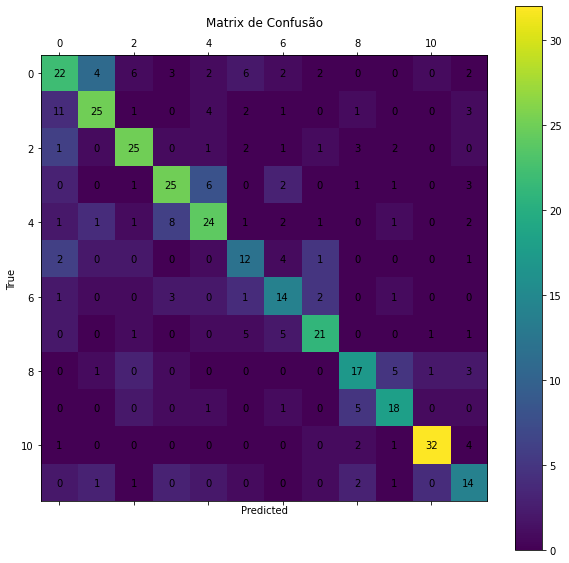
\includegraphics[width=1.1\linewidth]{experiments/svm_aug/confusion_matrix.png}
    \caption{Sem Augmentation}\label{fig:experiment_svm_aug}
  \end{minipage}\hfill
  \begin{minipage}{.47\textwidth}
    \centering
    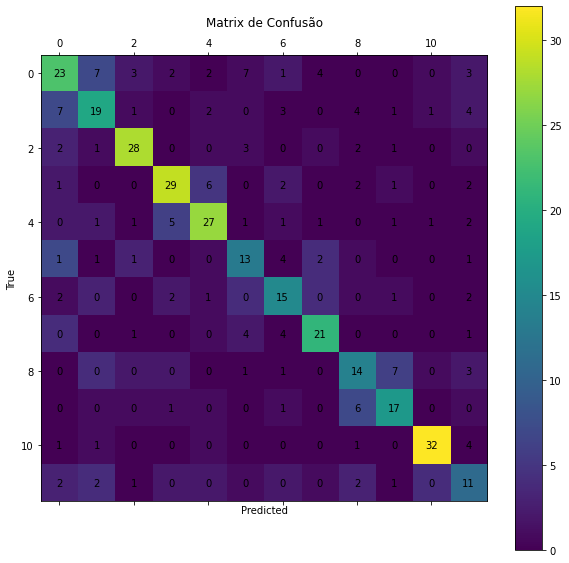
\includegraphics[width=1.1\linewidth]{experiments/svm_noaug/confusion_matrix.png}
    \caption{Com Augmentation}\label{fig:experiment_svm_noaug}
  \end{minipage}
\end{figure}

\begin{table}[!htb]
  \centering
  \begin{tabular}{|c|c|c|c|}
    \hline
    \textbf{Experimento} & \textbf{F1Score} & \textbf{Acurácia} & \textbf{Tempo de Execução (s)} \\ \hline
    svm\_aug             & 0.616            & 0.621             & 1992.622                       \\ \hline
    svm\_noaug           & 0.615            & 0.621             & 12.658                         \\ \hline
  \end{tabular}
  \caption{Resultados Obtidos (SVM)}
  \label{tab:experiment_svm}
\end{table}

\newpage

\section{Discussão dos Resultados}

A Tabela \ref{tab:summary} mostra a sumarização de todos os resultados obtidos nos experimentos.

\begin{table}[!htb]
  \centering
  \begin{tabular}{|c|c|c|c|}
    \hline
    \textbf{Experimento} & \textbf{Loss} & \textbf{Acurácia} & \textbf{Tempo de Execução (s)} \\ \hline
    lenet5\_noaug\_32    & 1.00          & 0.66              & 5.78                           \\ \hline
    lenet5\_noaug\_64    & 0.88          & 0.70              & 9.51                           \\ \hline
    lenet5\_noaug\_128   & 0.80          & 0.74              & 16.44                          \\ \hline
    default\_noaug\_32   & 0.83          & 0.71              & 12.37                          \\ \hline
    default\_noaug\_64   & 0.71          & 0.77              & 21.38                          \\ \hline
    default\_noaug\_128  & 1.03          & 0.76              & 40.14                          \\ \hline
    lenet5\_aug\_32      & 0.80          & 0.73              & 63.91                          \\ \hline
    lenet5\_aug\_64      & 0.84          & 0.72              & 105.89                         \\ \hline
    lenet5\_aug\_128     & 1.01          & 0.72              & 193.93                         \\ \hline
    default\_aug\_32     & 0.63          & 0.78              & 159.49                         \\ \hline
    default\_aug\_64     & 0.96          & 0.76              & 297.53                         \\ \hline
    default\_aug\_128    & 1.26          & 0.76              & 557.75                         \\ \hline
  \end{tabular}
  \caption{Sumários dos Obtidos}
  \label{tab:summary}
\end{table}

Nos experimentos realizados o foco não foi a otimização dos resultados de Acurácia, por este motivo, não foram exploradas alternativas ou ajustes de parâmetros.

Na implementação de Data Augmentation, é possível notar em algumas imagens, que o resultado gerado podem não corresponder exatamente a uma informação que ajude com características verdadeiras de uma determinada classo. Isso pode ter influenciado diretamente na melhoria dos resultados.

Por exemplo, é possível observar algumas anomalidas destacadas na Figura \ref{fig:image_months_wrong}.

\begin{figure}[!htb]
  \centering
  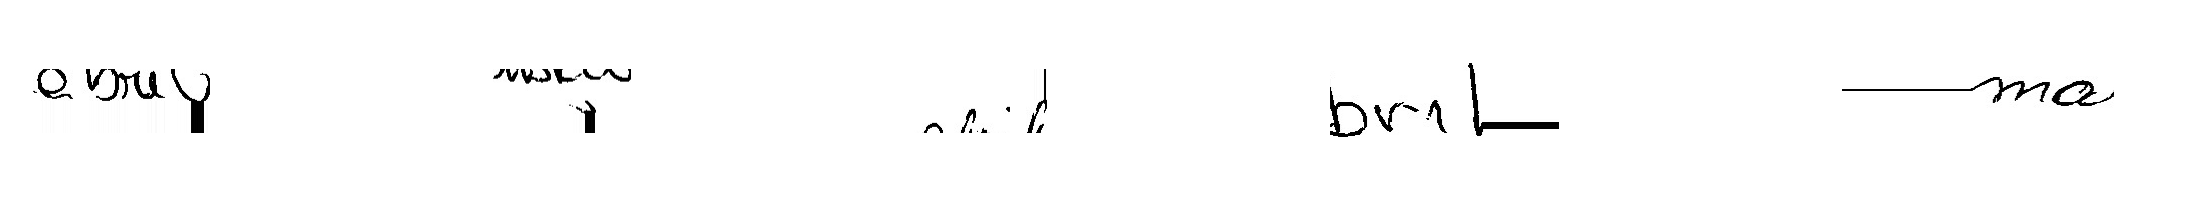
\includegraphics[width=35em]{images/image_months_wrong.png}
  \caption{Exemplos sem características verdadeiras}
  \label{fig:image_months_wrong}
\end{figure}

É possível notar que o melhor resultado foi obtido pelo experimento \textit{default\_aug\_32} com o valor de Acurácia = 0.78 e Loss = 0.63.

O pior resultado foi obtido pelo experimento \textit{lenet5\_noaug\_32} com o valor de Acurácia = 0.66 e Loss = 1.

Para os experimentos da modelo LeNet5 sem data augmentation, foi possível notar que os gráficos de acurácia e perda, se mantiveram bastante equilibrados, com a exeção da execução com 128 épocas na qual,após a época 20 o acurácia e perda se estabilizam. Quanto as matrizes de confusão, os erros se concentram praticamente nos mesmos lugares, pois os dados fonte são os mesmos. Os resultados melhoraram com os experimentos com mais épocas.

Para os experimentos da modelo LeNet5 com data augmentation, foi possível notar que os gráficos de acurácia e perda, tiveram uma distância considerável para 32 épocas; Para 64 épocas temos uma estabilidade após a época 50, que se mantém para o experimento de 128 épocas. Quanto as matrizes de confusão, os erros se concentram praticamente nos mesmos lugares, pois os dados fonte são os mesmos. Os resultados pioram com os experimentos com mais épocas.

Já para os experimentos do modelo personalizado sem data augmentation, foi possível notar que os gráficos de acurácia e perda, se mantiveram bastante equilibrados, e com uma estabilidade após época 20. Quanto as matrizes de confusão, os erros se concentram praticamente nos mesmos lugares, pois os dados fonte são os mesmos. Os resultados melhoraram com os experimentos com mais épocas.

E por fim, para os experimentos do modelo personalizado com data augmentation, foi possível notar que os gráficos de acurácia e perda, se mantiveram bastante equilibrados, e com uma estabilidade após época 20. Quanto as matrizes de confusão, os erros se concentram praticamente nos mesmos lugares, pois os dados fonte são os mesmos. Os resultados pioram com os experimentos com mais épocas.

A Tabela \ref{tab:experiment_svm_final} mostra os resultados de F1Score, Acurário e o tempo de execução obtidos nos experimentos relacionados ao SVM. É possível notar que não houve melhora nos resultados, provavelmente por conta da qualidade das imagens geradas pela técnica de data augmentation.

\begin{table}[!htb]
  \centering
  \begin{tabular}{|c|c|c|c|}
    \hline
    \textbf{Experimento} & \textbf{F1Score} & \textbf{Acurácia} & \textbf{Tempo de Execução (s)} \\ \hline
    svm\_aug             & 0.616            & 0.621             & 1992.622                       \\ \hline
    svm\_noaug           & 0.615            & 0.621             & 12.658                         \\ \hline
  \end{tabular}
  \caption{Resultados Obtidos (SVM)}
  \label{tab:experiment_svm_final}
\end{table}

\newpage

\section{Código Fonte}

Os códigos fonte podem ser encontrados em:

\begin{itemize}
  \item GitHub: https://github.com/diogocezar/phd-machine-learning-lab3
  \item Google Colab: https://bit.ly/3gR739z
\end{itemize}

\end{document}